\documentclass[titlepage]{article}
\usepackage{graphicx}
\usepackage{amsmath}
\usepackage[T1]{fontenc}  
\usepackage[utf8]{inputenc}   
\usepackage{geometry}
\usepackage{caption}
\usepackage{hyperref}
\usepackage{tabularx,ragged2e,booktabs,caption}
\newcolumntype{C}[1]{>{\Centering}m{#1}}
\renewcommand\tabularxcolumn[1]{C{#1}}
\usepackage[font=small,labelfont=bf]{caption}
 \geometry{
 a4paper,
 total={210mm,297mm},
 left=20mm,
 right=20mm,
 top=20mm,
 bottom=20mm,
 } 
\usepackage{eso-pic}
\AddToShipoutPicture{%
  \AtPageUpperLeft{%
    \hspace*{20pt}\makebox(200,-20)[lt]{%
      \footnotesize%
      \textbf{Lucas Hellström}%
}}}




\title{Using TTV signals to find and catalogue multi-planet systems}
\author{Lucas Hellström\\ \small{nat14lhe@student.lu.se}}
\date{}

\begin{document}
\maketitle

\section{Introduction}
	By measuring Transit Timing Variations, TTVs, it is possible to separate a single-planet system from a multi-planet system. This is done by measuring the time the planet takes to make one complete revolution around its host star. If the time for one revolution differs by a non-negligible amount the system can be further observed to confirm the existents of multiple planets around the star. 
	
	In this paper, it will be argued that the use of TTVs to detect exoplanets plays a fundamental role in our discovery of distant worlds. An objective of the study was to investigate transit times measured by the Kepler satellite and, by specifying a number of parameters, simulate the data that the upcoming TESS satellite will produce. This data is analysed to get a better understanding of multi-planets systems and to create a catalogue of these systems for further study. 
	
	
\section{Theory}
	The easiest obtainable information about a star far way is the intensity of the star. By measuring this over some time a light curve can be made which describes the intensity of the star over some time. If there is a decrease in the intensity in regular intervals one or more planets might be transiting. A transit is a phenomenon where a planet moves between a star and the observer causing the intensity to decrease by blocking some of the light emitted by the star. This can be seen in figure \ref{fig:trans}
	
	\begin{figure}[h!]
		\centering
		\captionsetup{justification=centering}
		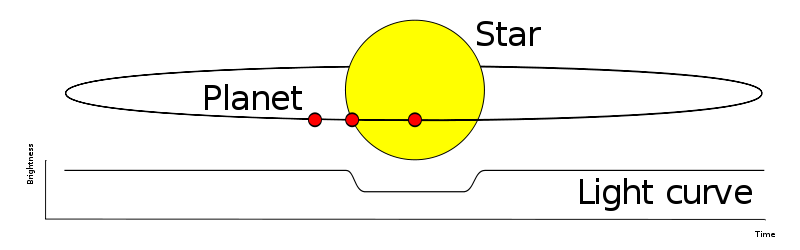
\includegraphics[width=0.6\textwidth]{planTrans.png}
		\caption{Illustration of a transiting planet and the resulting light curve. \\  \small{ Source: \url{https://commons.wikimedia.org/wiki/File:Planetary_transit.svg}}}
		\label{fig:trans}
	\end{figure}\
	When measuring a transiting planet the time between two transits might differ. The cause of this is most probably an outer heavier planet pulling the inner planet, accelerating or decelerating it depending on the relative position of the planets. As at least two planets are required for TTVs to show the conclusion can be drawn that if TTVs are measured the system consists of at least two planets. This method of detecting planets is useful as it can contain planets that is not transiting, that is that they are never positioned between the star and the observer. This is important as most planets are not transiting their stars. The probability for a transit is approximately 
	\begin{equation}
		P = \frac{R_{\star}}{a}
	\end{equation}
	Where P is the probability of a transit, $R_{\star}$ is the radius of the star and $a$ is the semi-major axis of the orbiting planet which for a circular orbit is the same as the radius of the orbit.\footnote{\url{http://curious.astro.cornell.edu/physics/77-the-universe/extrasolar-planets/general-questions/211-how-likely-is-it-for-a-planet-to-transit-its-star-intermediate}} This equation shows that for a Sun-like star a planet with a small orbit will have an approximately 10$\%$ chance of transiting. This decreases for planets further out and for a planet at a distance equal to the distance between the Earth and the Sun the probability is only $0,47\%$. With these numbers in mind it is easy to see the advantage of being able to detect planets around a star where only one planet is transiting.
	
	In order to obtain TTV signals a program called TTVFast \footnote{\url{https://github.com/kdeck/TTVFast}} is used. It accepts a number of input parameters, simulates a solar system and outputs the respective transit times for that system. This is preferred over normal measurements by telescope as it allows the user to specify the input parameters and also reduces the cost of measurement significantly. To obtain a satisfactory number of transit times a telescope would need to observe the system for a long time.
	
	In order to obtain data of distant stars a telescope on the ground is often not enough. This is due to light pollution, although this for the most part be avoided by choosing a position with generally low light pollution. Another thing that makes ground based telescopes inferior is the atmosphere. When light goes through the atmosphere it is scattered. Different wavelengths are scattered differently, which is the cause of the red Sun at sunset and sunrise, which may distort the very sensitive ground based telescopes. To solve this problem space based telescopes are used. The most important is the Kepler telescope, launched in 2009, which has since its launch discovered over 1000 confirmed exoplanets, more than any other mission to this date.\footnote{\url{https://www.nasa.gov/press-release/nasas-kepler-mission-announces-largest-collection-of-planets-ever-discovered}}
	
	An upcoming mission will include the Transiting Exoplanet Survey Satellite, or TESS for short, and have a planned launch in spring 2018. TESS will look for transiting planets but the main difference between it and Kepler is that Kepler studied one point for a very long time while TESS will study one sector in the sky for 27 days and then turn to another sector. By doing this it will look at the whole sky during its two years mission duration. The data from TESS is what this paper will analyse although as it will not be available during the project duration Kepler data will be used and modified to simulate TESS data.
	
\section{Method}
	The data for this project is obtained from the exoplanet archive run by NASA, modified to be in a format compatible with TTVFast. The output from TTVFast is different transit times which are fitted with a linear fit which is subtracted to remove background and noise. 
	
	To simulate TESS data from Kepler data a number of things need to be considered. The first thing is that Kepler studied far fewer stars than TESS will and thus the number of systems is drastically reduced for Kepler data. To account for this a paper written by Sullivan et al. \footnote{\url{http://iopscience.iop.org/article/10.1088/0004-637X/809/1/77/pdf}} is used. The Sullivan paper simulates TESS data which is compared to Kepler data to obtain a catalogue of systems which can be analysed by TTVFast. To obtain the time that TESS will study each system a tool made by the TESS GI team\footnote{\url{https://heasarc.gsfc.nasa.gov/cgi-bin/tess/webtess/wtm.py}} is used. This combined with the Sullivan data is enough to run TTVFast for a large number of potential systems.
	
	The data from TTVFast is analysed by looking at the amplitude of the TTVs, that is the difference in time one transit takes. An amplitude of over $0.1$ minutes is used to separate real systems and false positives.
\section{Results}
	The results is in the form of a catalogue of multi-planet systems not yet complete. An example of a transit curve where a TTV signal is seen can be found in figure \ref{fig:TTV}
	
	\begin{figure}[h!]
		\centering
		\captionsetup{justification=centering}
		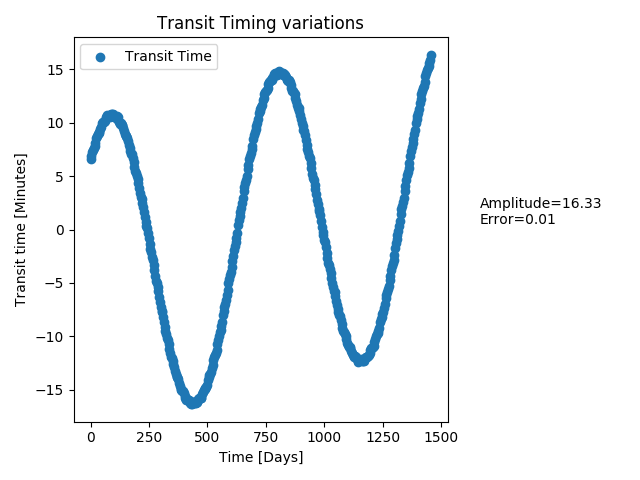
\includegraphics[width=0.6\textwidth]{K00221.png}
		\caption{Figure of a TTV signal curve where the time for one transit is plotted against the time of the observation since the beginning of the mission}
		\label{fig:TTV}
	\end{figure}\
\section{Discussion}
	From the results obtained so far it can be seen that some systems show significant TTV signals while other systems does not show any at all. One reason for this can be that the inner most planets which is studied is heavier than the other most planets. This creates a situation where the outer planet is not heavy enough to pull the inner planet enough for any significant signal to show. Another reason might be that the ration between the transit times for the planets in the system is a particular value where the gravitational pull cancels out and no signal is seen.
	
	
	For todays society this project will not have much value. On the other hand it will be able to simplify future projects where a catalogue of potential multi-planet systems are required. If future project requires looking at a number of multi-planets systems over a long time it is significantly easier to find a catalogue of potential systems then to search blindly after them with the help of a telescope.

\end{document}

